\chapter{System Design}

\section{Relational Table Description}
The RideShare relational database comprises seven strictly normalized relations, engineered to eliminate redundancy, uphold domain constraints, and enforce referential integrity across all platform operations, as summarized in Table~\ref{tab:schema}:

\begin{table}[H]
\centering
\small
\caption{RideShare Relational Schema Specification}
\label{tab:schema}
\begin{tabular}{|p{2.0cm}|p{2.2cm}|p{4.8cm}|p{4.8cm}|}
\hline
\rowcolor{headerblue}
\color{white}\textbf{Relation} & \color{white}\textbf{Primary Key} & \color{white}\textbf{Foreign Keys / Unique Constraints} & \color{white}\textbf{Key Attributes} \\
\hline
\rowcolor{rowgray}
\texttt{locations} & \texttt{name [PK]} & --- & \texttt{latitude, longitude} \\
\hline
\texttt{users} & \texttt{user\_id [PK]} & \texttt{email [UNIQUE]} & \texttt{name, number} \\
\hline
\rowcolor{rowgray}
\texttt{drivers} & \texttt{driver\_id [PK]} & --- & \texttt{driver\_name, phone\_no, license\_no, ratings} \\
\hline
\texttt{vehicles} & \texttt{vehicle\_id [PK]} & \texttt{driver\_id [FK, UNIQUE $\rightarrow$ drivers] [1:1]} & \texttt{vehicle\_number, vehicle\_type, capacity} \\
\hline
\rowcolor{rowgray}
\texttt{rides} & \texttt{ride\_id [PK]} & \texttt{user\_id [FK], driver\_id [FK], pickup [FK], dropoff [FK]} & \texttt{ride\_date, fare, ride\_status, ride\_type, passengers\_count} \\
\hline
\texttt{payments} & \texttt{payment\_id [PK]} & \texttt{ride\_id [FK, UNIQUE $\rightarrow$ rides] [ON DELETE CASCADE]} & \texttt{payment\_mode, amount, payment\_status} \\
\hline
\rowcolor{rowgray}
\texttt{reviews} & \texttt{review\_id [PK]} & \texttt{user\_id [FK $\rightarrow$ users]} & \texttt{comments, rating [CHECK 1..5]} \\
\hline
\end{tabular}
\end{table}

\section{Relational Schema Architecture}
The overall schema connectivity and constraint pathways are visualized in Figure~\ref{fig:schema_diagram}, illustrating foreign key mappings, cardinality constraints, and cascade relationships between the seven core relations.

\begin{figure}[H]
\centering
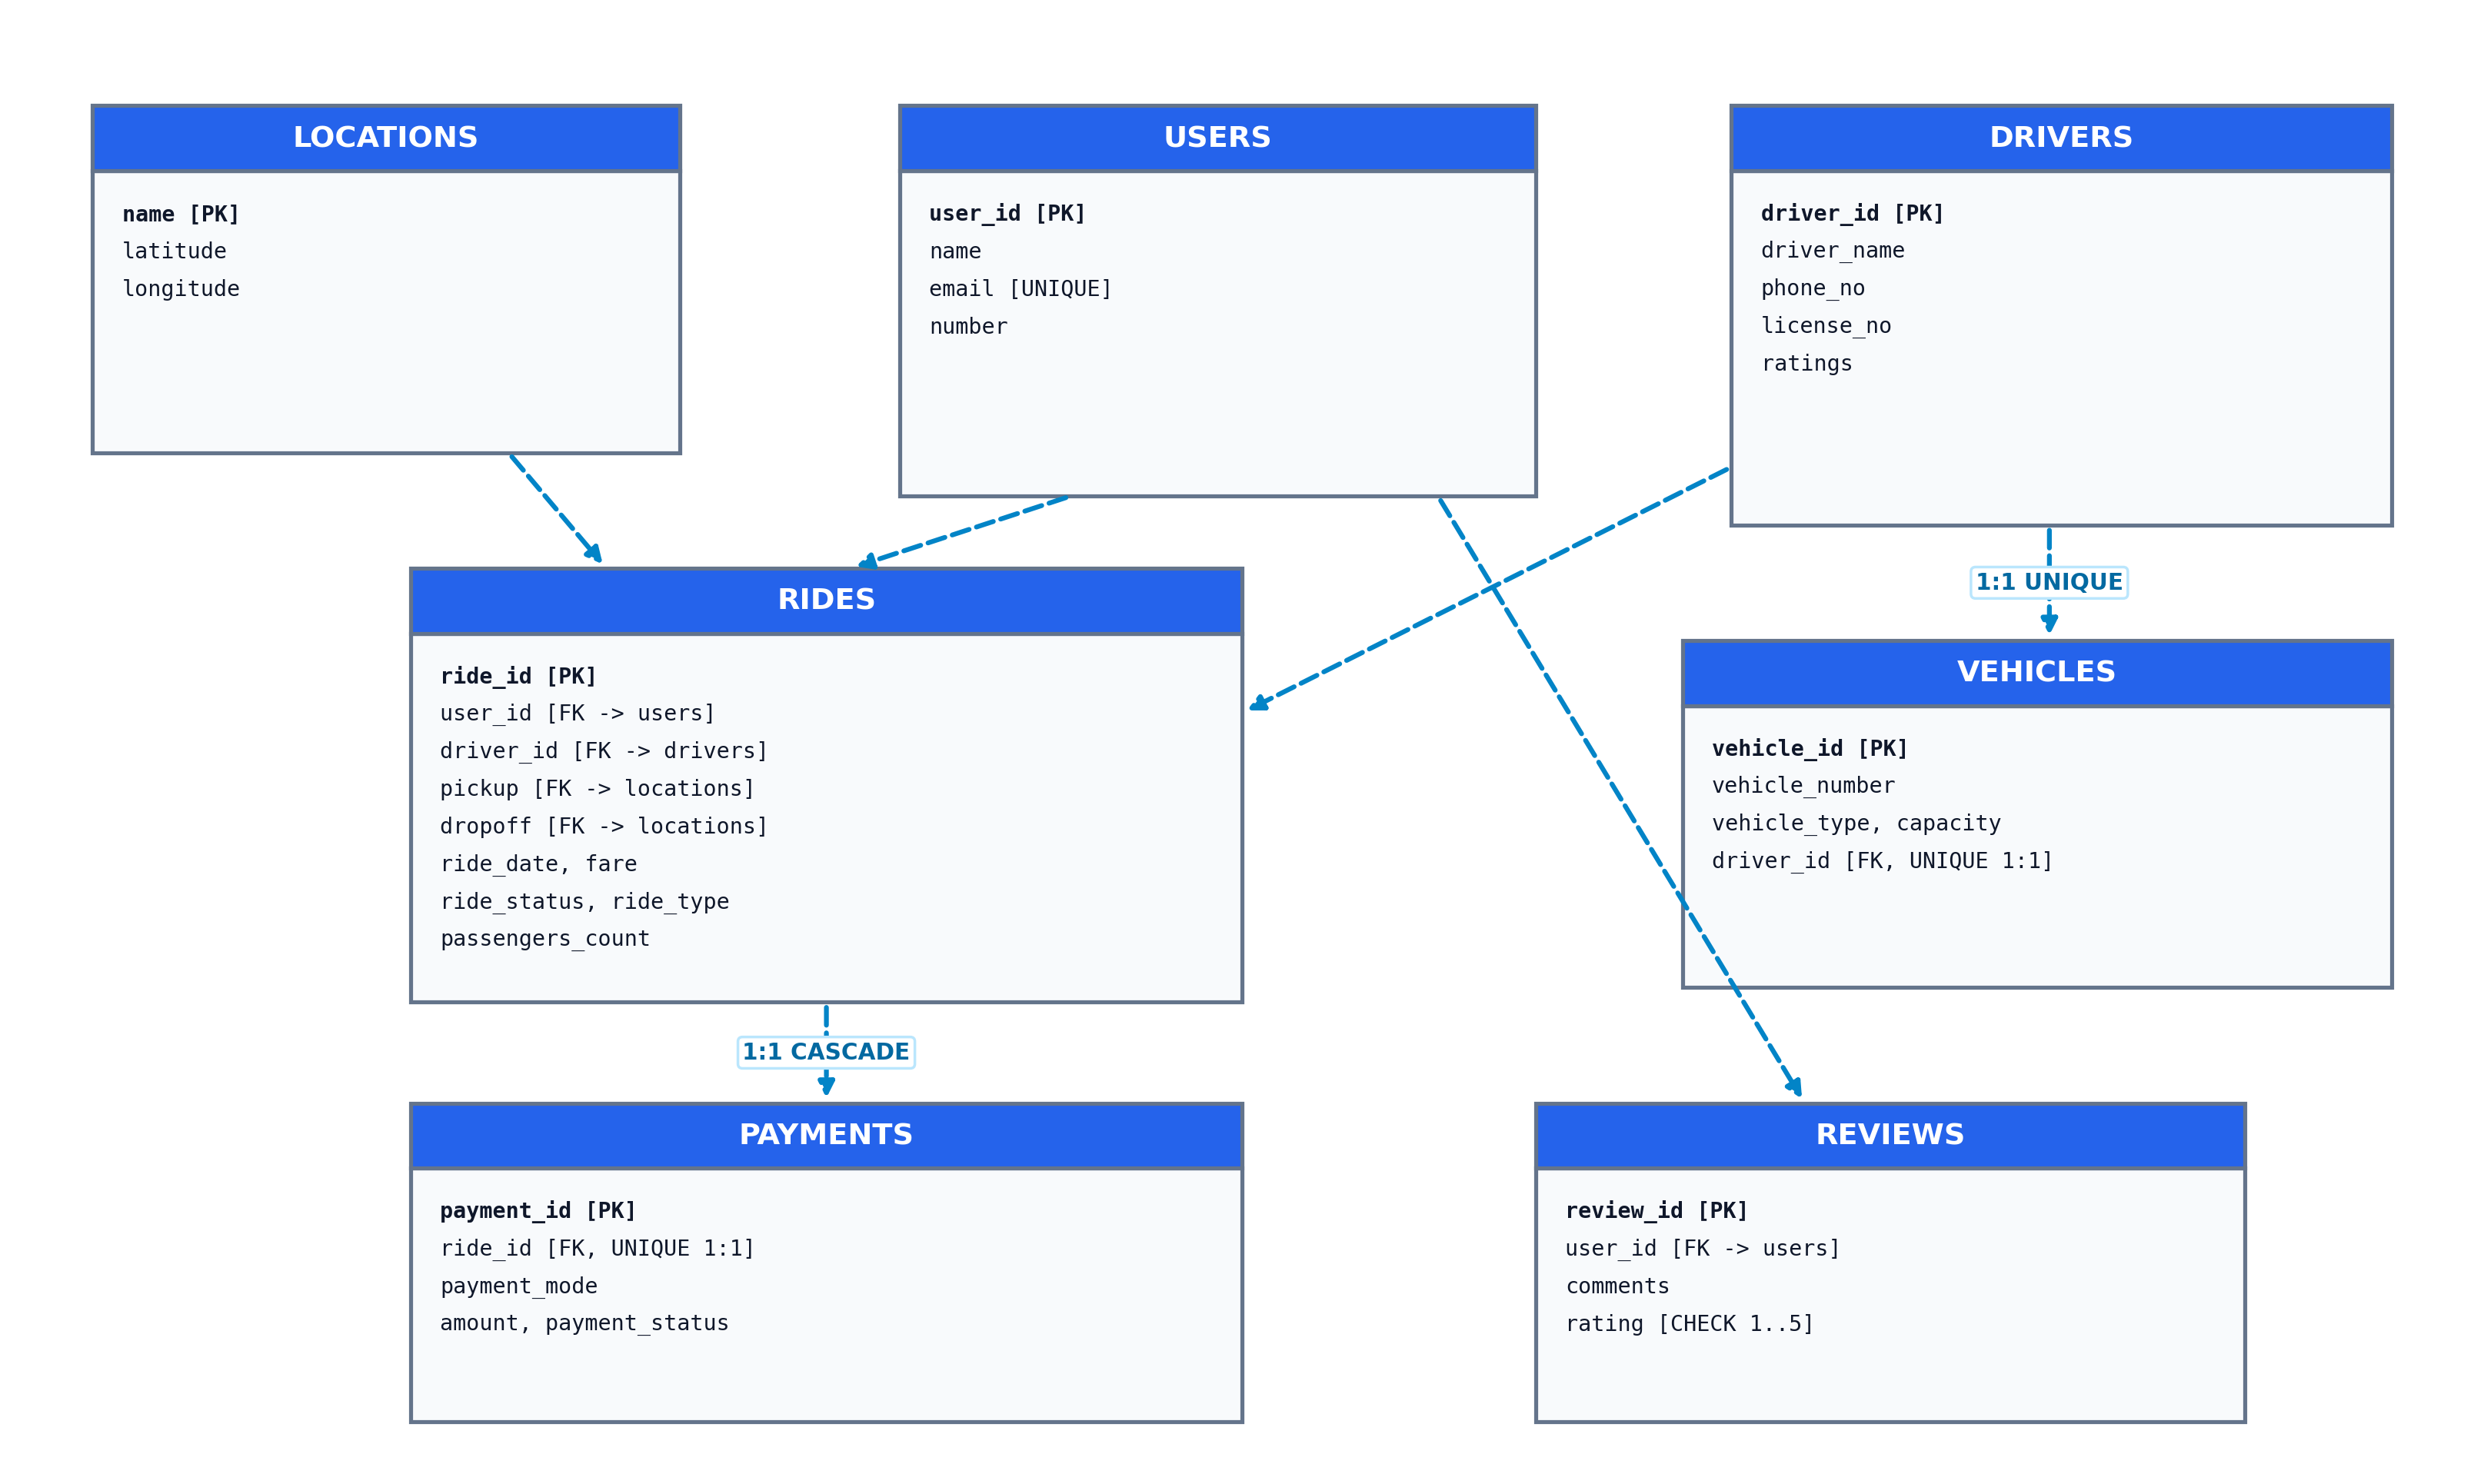
\includegraphics[width=0.82\textwidth]{images/schema_diagram.png}
\caption{Relational Schema Architecture Model with Keys \& Constraints}
\label{fig:schema_diagram}
\end{figure}

\clearpage

\section{Entity-Relationship Diagram (Chen Notation)}
The conceptual data model for the RideShare system was developed using formal Chen notation \cite{chen1976}, as illustrated in Figure~\ref{fig:er_diagram}:

\begin{figure}[H]
\centering
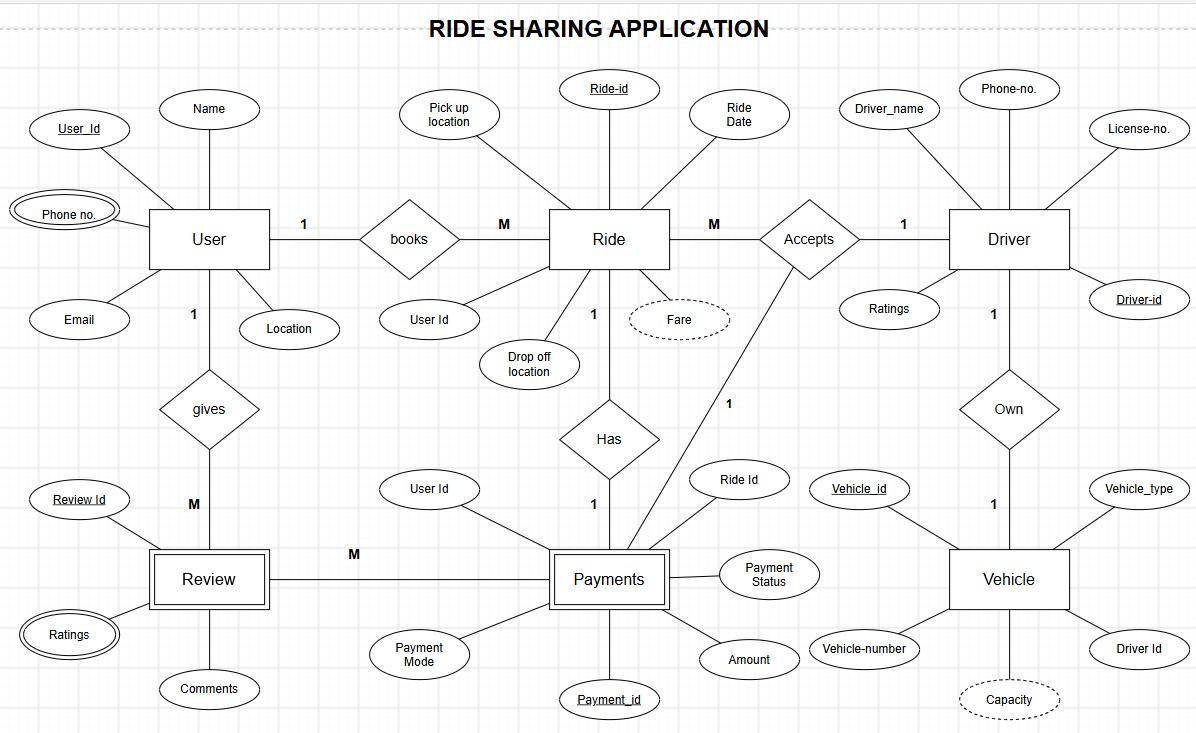
\includegraphics[width=0.80\textwidth]{images/er_diagram_crisp.png}
\caption{Formal Chen-Notation Entity-Relationship Diagram for RideShare}
\label{fig:er_diagram}
\end{figure}

\textbf{Chen Notation Specification \& Cardinality Constraints:}
\begin{itemize}[itemsep=1pt, topsep=1.5pt, parsep=0pt]
    \item \textbf{Strong Entity Sets:} \texttt{User}, \texttt{Driver}, \texttt{Vehicle}, \texttt{Ride}, each identified by a surrogate primary key.
    \item \textbf{Weak Entity Sets:} \texttt{Payments} (dependent on \texttt{Ride}) and \texttt{Review} (dependent on \texttt{User}).
    \item \textbf{Multivalued Attribute:} \texttt{Phone no.} on \texttt{User} and \texttt{Driver}, decomposed to ensure 1NF conformity.
    \item \textbf{Derived Attribute:} \texttt{Fare} on \texttt{Ride}, dynamically evaluated via server-side Haversine computation.
    \item \textbf{Relationships \& Cardinalities:} \texttt{books} ($1:M$), \texttt{accepts} ($1:M$), \texttt{owns} ($1:1$ \texttt{UNIQUE}), \texttt{has} ($1:1$ with \texttt{CASCADE}), and \texttt{gives} ($1:M$).
\end{itemize}

\section{Relational Schema \& Normalization Analysis}
\textbf{Relational Schema (Bracket Notation):}
\begin{itemize}[itemsep=1pt, topsep=1.5pt, parsep=0pt]
    \item \texttt{locations}(\underline{name [PK]}, latitude, longitude)
    \item \texttt{users}(\underline{user\_id [PK]}, name, email [UNIQUE], number)
    \item \texttt{drivers}(\underline{driver\_id [PK]}, driver\_name, phone\_no, license\_no, ratings)
    \item \texttt{vehicles}(\underline{vehicle\_id [PK]}, vehicle\_number, vehicle\_type, capacity, driver\_id [FK, UNIQUE])
    \item \texttt{rides}(\underline{ride\_id [PK]}, user\_id [FK], driver\_id [FK], pickup\_location [FK], dropoff\_location [FK], ride\_date, fare, ride\_status, ride\_type, passengers\_count)
    \item \texttt{payments}(\underline{payment\_id [PK]}, ride\_id [FK, UNIQUE], payment\_mode, amount, payment\_status)
    \item \texttt{reviews}(\underline{review\_id [PK]}, user\_id [FK], comments, rating)
\end{itemize}

\textbf{Normalization Analysis:}
\begin{itemize}[itemsep=1pt, topsep=1.5pt, parsep=0pt]
    \item \textbf{First Normal Form (1NF):} All attribute values are strictly atomic; multivalued phone numbers are decomposed into distinct attributes.
    \item \textbf{Second Normal Form (2NF):} Every relation employs a single-attribute surrogate primary key, eliminating partial functional dependencies.
    \item \textbf{Third Normal Form (3NF):} Transitive functional dependencies are eradicated by factoring spatial coordinates into \texttt{locations}.
    \item \textbf{Boyce-Codd Normal Form (BCNF):} For every non-trivial functional dependency $X \rightarrow Y$, the determinant $X$ is a superkey.
\end{itemize}